\chapter{Introduction}
This project is about machine learning of different statistical classifiers.
Machine learning is about construct and study systems that can learn from data.
This could be used to train a system to recognize patterns in, for instance, emails and learn how to distinguish between spam and non-spam messages. In this project the classifiers are applied to reviews and the task is to categorize these.
By statistical analysis of experiments, the classifiers are compared in terms of, for instance, classification accuracy.

\section{Problem description}
The problem is to categorize reviews from Amazon in 6 different categories; books, camera, DVD, health, music and software.
The classification is done by implementing five different classification algorithms; Naive Bayes, Perceptron, Averaged Perceptron, K-nearest neighbours (KNN) and Support vector machine (SVM). \\\\
There is three different kinds of classification tests that should be done: 
\begin{itemize}
\item In-domain sentiment analysis - For each category, train and classify documents as positive or negative
\item Out-of-domain sentiment analysis - Train on one category and test on another
\item Text categorization - categorize the documents into their categories
\end{itemize}
Before classifying the input data, which is text files, must be processed.
The input should be divided in words somehow, either one word (unigrams) or two words (bigrams). Some common words are totally useless for the classification, such as ''the'' and ''I''. These are called stop-words and should not be a part of the input to the algorithms. To get less words it's also possible to use a stemmer, such as Snowball to prevent separation of different inflectional forms, such as ''person'' and ''persons''. Another way of getting less input data is to use Term Frequency–Inverse Document Frequency TF-IDF. TF-IDF is a numerical statistic of how important a is in a document.

\section{Theory}
Describe briefly the scientific papers or book chapters you found relevant to the problem, references to sec 6. Explain which are relevant for your project and which not and why.
\subsection{Text classification}
One part of supervised learning is the field Text classification which is to classify documents into a fixed number of predefined categories. The categories could be sentimental (positive / negative) or different topics that the document concern. 

\subsubsection{Representing text}
A document is typically a huge string containing all characters and is not suitable for classification, hence some processing needs to be done on each document. 
\\\\
All words in a document isn't interesting when doing text classification. E.g. words like "the", "one", "are", "is" are words that will occur in any human readable text, but has no value when trying to find similarities and differences between documents. These words are called "stop-words" and are usually filtered out and treated as noise. 
\\\\
When working with document we want to treat different inflections(?) of a word as the same word. There is no need to separate the words "persons" and "person", because both words give us the same information we want. This is called Stemming and we will not focus more on the theory behind it.
\\\\
There are various ways of storing document and the representation has a big impact on the result of different classifiers. The Bag-of-words model is a simplifying model where a text is represented as a unordered set of words, without respect to grammar or order of words. 
\\\\
Build a feature vector which is an n-dimensional vector of numerical features that represents the words.
\subsubsection{Features}
\textbf{Feature-size} \\
\textbf{n-gram} \\
\textbf{TF-IDF} \\
\textbf{Wordcount} 
Count the number of occurrences of each word or calculating the tf-idf, term frequency–inverse document frequency, of each word. 
\begin{equation*}
\begin{array}{l}
tf(t,d) = \frac{f(t,d)}{(max \{f(w,d) : w \in d\})} \\
idf(t,D) = log(\frac{|D|}{|\{d \in D : t \in d\}|})
\end{array}
\end{equation*}
\\\\


\subsection{Naive Bayes}
The Naive Bayes classifier uses (naive) independence assumptions to simplify the conditional probability $P(c\vert\mathbf{x})$ of a feature vector $\mathbf{x} \in \mathbb{R}^D$ belonging to class $c$ by using Bayes' rule to formulate $P(c\vert \mathbf{x}) = \frac{P(\mathbf{x}\vert c) P(c)}{P(\mathbf{x})}$ and rewriting as follows.
\begin{align*}
P(c\vert \mathbf{x}) &\propto P(\mathbf{x}\vert c)P(c)
\\&=P(c,\mathbf{x})
\\&\propto P(c) P(x_1,...,x_D\vert c)
\\&\propto P(c) P(x_1\vert c) P(x_2,...,x_D\vert c, x_1)
\\&\propto P(c) P(x_1\vert c) P(x_2\vert c, x_1) P(x_3,...,x_D\vert c,x_1,x_2)
\\&\propto P(c) P(x_1\vert c) P(x_2\vert c, x_1) P(x_3\vert c,x_1,x_2) \dots P(x_D\vert c, x_1,...,x_{D-1})
\\&\dots
\end{align*}
The independence assumption says that each feature $x_i$ is independent of every other feature $x_j,...x_k$, rendering $P(x_i\vert x_j,...,x_k) = P(x_i\vert c)$, which translates the posterior $P(c\vert \mathbf{x})$ to
\begin{align}
P(c\vert \mathbf{x}) &\propto P(c) P(x_1\vert c) P(x_2\vert c) \dots P(x_D\vert c) \nonumber
\\&= P(c) \prod_{i=1}^{D} P(x_i\vert c).\label{eq:naivebayes_model}
\end{align}
A suitable choice for each conditional distribution $P(x_i\vert c)$ is the \textit{maximum likelihood estimate}, MLE, which corresponds to the relative frequency of each parameter in the training data.

The classification procedure then calculates the \textit{maximum a posteriori} (MAP) class $c_{\textit{map}} = \argmax_{c\in C} P(c\vert \mathbf{x})$. Since the argument $c$ that maximizes $P(c\vert \mathbf{x})$ also maximizes $\log P(c\vert \mathbf{x})$, the product in equation \ref{eq:naivebayes_model} can be written as a sum of log terms, which helps to avoid arithmetic underflow. The pseudocode for the classification procedure is shown in Algorithm \ref{algorithm:naive_bayes_classification}.

\begin{algorithm}[h]
\label{algorithm:naive_bayes_classification}
 \SetAlgoLined
 \SetKwInOut{Input}{input}\SetKwInOut{Output}{output}
 \KwData{\textit{Feature vector with unknown class} $\mathbf{x} \in \mathbb{R}^D$; \textit{Class weights} $\{P(c) : c \in C\}$; \textit{Conditional feature probabilities} $\{P(x_1\vert c), ..., P(x_D\vert c)\}$}
 \KwResult{Classification for $\mathbf{x}$}
 \ForEach{$c \in C$}
 {
 	score[$c$] $\leftarrow \log P(c)$\\
 	\For{$i=1$ \KwTo $D$}
 	{
 		score[$c$] += $\log P(x_i\vert c)$
 	}
 }
 \Return $\displaystyle \argmax_{c \in C} score[c]$ \\

 \caption{Multinomial Naive Bayes classification algorithm}
\end{algorithm}

\subsection{K-Nearest Neighbour (KNN) algorithm}
%http://www.cse.chalmers.se/edu/course/TDA231/mlsli11.pdf
K-nearest neighbors (KNN) algorithm is one of the simplest machine learning
algorithms. The classification performed by KNN works as follows: Fix some
number $k$. For any new $x \in X$, take the most common classification value among
the $k$ training examples in $D$ closest to $x$.
\\\\
Even though the KNN algorithm
seems extraordinary simple there are some things that one must take in
consideration. First of all what is nearest? There is of course a natural
distance function in a geometrical space but a proper definition in parameter
space is not obvious. As it turn out a distance function can be defined in a lot
of ways. The given attributes are overall very different in reality.
One may may multiply each attribute variable by arbitrary factors or in other
words stretch the coordinate axes arbitrary and independent. It is very easy to
find examples when doing so will result in very different outcomes of the classifications.
Even further irrelevant attributes may change the classification even though they
shouldn't do so. This phenomena is called \emph{curse of dimensionality}. One
can try to find good stretch factors by performing cross validation.
One takes a vector of stretch factors that
minimizes the classification errors on a valid set. The back side is that
this will require a lot of test vectors.
\\\\
An other problem is the computation complexity. KNN is sad to have a lazy
learning method. In other words it does output hypotheses in explicit form.
Instead a lot of computational steps are required for the classification.
\\\\
A further issue is to find a suitable $k$. A great choose of $k$ various
depending on many circumstances. A keystone is that if the training set is large
it's important get rid of noise in the data hence increase $k$. On the other
hand a big $k$ requires more calculation. There are however also other more
complex ways for reducing noise.
%https://dl.dropbox.com/u/5139428/ml-course/Classification1.pdf
\begin{center}
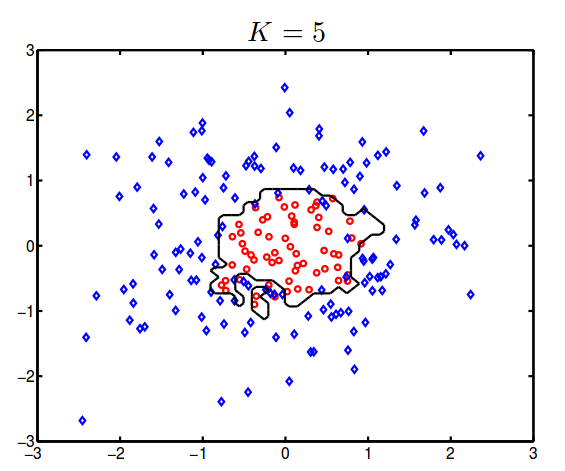
\includegraphics[scale=0.5]{fig/KNN.png}
\end{center}

\subsection{Support Vector Machine (SVM)}
Support Vector Machines (SVM) constructs a non-probabilistic linear classification separating two different classes of input data. 
\\\\
Given some input data SVM outputs a hyperplane which is a separating the given data depending on its class. SVM chooses the hyperplane which has the largest distance to the nearest training data point of any class, this distance is refered to as the margin and denoted $\gamma$. In general the larger margin, the lower generalization error. (Motivera!) 
\\\\
By default SVM is so-called hard margined, meaning that all points must be on correct side of the hyperplane. 
\\\\
The data points that is at the margin distance from the hyperplane is called the support vectors. The hyperplane only depends on the support vector, meaning that SVM is dimensional independent (??). This is shown in Figure~\ref{fig:svm}.
\\\\
SVM can perform classification on both linear and non-linear input data. Classification on non-linear data can be performed by mapping the data into a high-dimensional feature space, through a kernel function. Different popular kernel functions are linear kernel, quadratic kernel, polynomial kernel and Gaussian radial basis function kernel (rbf). (förklara dessa!)
\\\\
SVM algorithm is closely related to the Perceptron algorithm with the difference that the hyperplane constructed by SVM maximizes the margin whilst perceptron is non-deterministic and returns a hyperplane which separates the input data. 
\begin{figure}[h!]
\centering
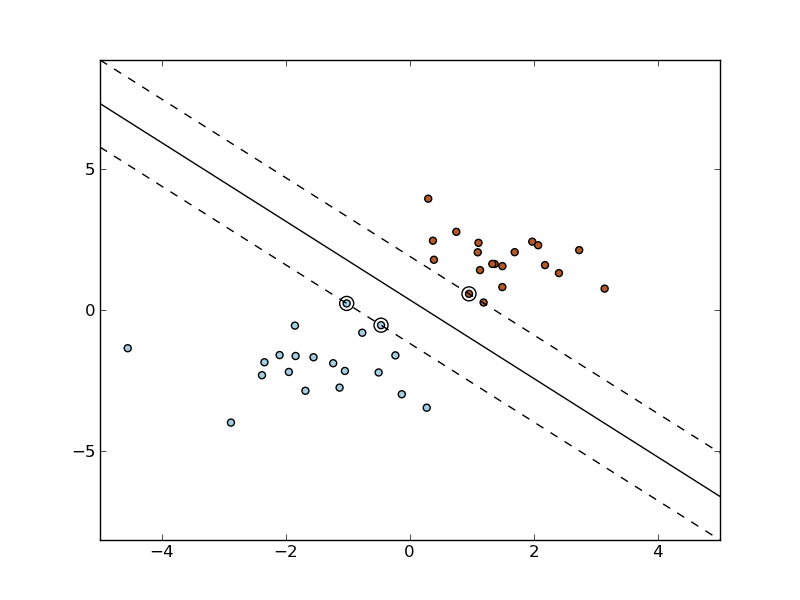
\includegraphics[scale = 0.5]{fig/svm_example_stolen.png}
\caption{Example of a classification by SVM. Support vecotors are marked with dots. \citep{svm_picture}}
\label{fig:svm}
\end{figure}
(Behövs det nämnas dual problemet och de matematiska?? Det finns material för det) 
\subsection{The Perceptron algorithm}
Perceptron is a linear, non deterministic, supervised classification algorithm. The Perceptron algorithm consider a 0/1 classification problem. \citep{perceptron_ai}
The algorithm tries to separate the input data with a linear decision boundary, i.e. tries to fit a hyperplane between the datasets. \citep{perceptron_url} This is shown in Figure~\ref{fig:perceptron}. The algorithm output a weight vector which represent the hyperplane between the two separated classes for each input data point. \citep{perceptron_url}
\begin{figure}[h!]
\centering
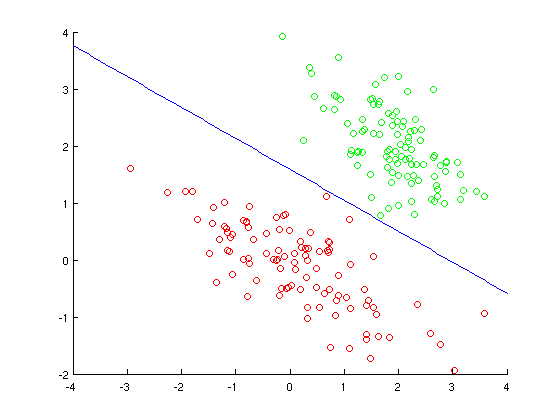
\includegraphics[scale = 0.5]{fig/perceptron_example.png}
\caption{Example of a classification by Perceptron}
\label{fig:perceptron}
\end{figure}\\
The basic idea for the Perceptron algorithm is for all input data, whose labeling are known, check their classification with the current weight vector. If the classification is correct, continue, else update the weight vector, $w$, according to Equation~\ref{eq:perceptron}. \citep{perceptron_ai}
\begin{equation}
\label{eq:perceptron}
w = w + (x \cdot y)
\end{equation}
where $x$ is the input data and $y$ the desired output (1 or -1). The Perceptron algorithm converge when the weight vector remains unchanged. \citep{perceptron_ai} New data is classified by Equation~\ref{eq:new_perceptron}.
\begin{equation}
\label{eq:new_perceptron}
class = sign(testData \cdot w)
\end{equation}
Where $class$ is the class the new data belongs to (1 or -1) and $w$ is the weight vector.\\\\
There is also another variant of the Perceptron algorithm, which is called Averaged Perceptron. They work in the same way, except that the Averaged Perceptron outputs the averaged weight vector instead of the final one.
\subsection{Text categorization}


\subsection{Programs and tools}
What tools and programs are already available for the problem, or for closely related ones?
Describe these briefly. Say how you can use them, and how your work will build on them, or differ from them. Explain which are relevant for your project and which not and why.
\\\\
* vilka program är vettiga att använda? -leta upp några-fördelar/nackdelar
skriv att vi valde matlab och varför.



